\lab{Algorithms}{The Shooting Method for Boundary Value Problems}{The Shooting Method for Boundary Value Problems}
\label{lab:Shooting}

Consider a boundary value problem of the form 
\begin{align}
	\label{shooting_bvp}
	\begin{split}
y'' &= f(x,y,y'), \quad a \leq x \leq b, \\
y(a) &= \alpha, \quad y(b) = \beta. 
\end{split}
\end{align}
One natural way to approach this problem is to study the initial value problem (IVP) associated with this differential equation: 
\begin{align}
	\label{shooting_ivp}
	\begin{split}
y'' &= f(x,y,y'), \quad a \leq x \leq b, \\
y(a) &= \alpha, \quad y'(a) = t. 
	\end{split}
\end{align}
The goal is to determine an  appropriate value $t$ for the initial slope, so that the solution of the IVP is also a solution of the boundary value problem. 

Let $y(x,t)$ be the solution of \eqref{shooting_ivp}. We wish to find a value of $t$ so that 
$y(b,t) - \beta = 0$. 
Applying Newton's method to the function $f(t) = y(b,t) - \beta$, we obtain the iterative method 
\begin{align*}
	t_{n+1} &= t_n - \frac{ f(t_n)}{f'(t_n) }, \\
	&= t_n - \frac{ y(b,t_n) - \beta}{\frac{d}{dt} \left.y(b,t)\right|_{t_n} },\quad n = 0,1,\ldots .
\end{align*}

We recall that Newton's method requires a good initial guess $t_0$; a plausible initial guess would be the average rate of change of the solution across the entire interval, so that $t_0 =  (\beta - \alpha)/(b-a)$. If this initial guess is not sufficient, the initial guess may be refined by looking at the solution $y(x,t_0)$ of the initial value problem.

This method requires us to evaluate or approximate the function $\frac{d}{dt} \left.y(b,t)\right|_{t_n}$. This term may be approximated with a finite difference, giving us the iterative method
\[t_{n+1} = t_n - \frac{ (y(b,t_n) - \beta)(t_n - t_{n-1})}{y(b,t_n) - y(b,t_{n-1}) }, \,\, n = 1, 2,\hdots .\]
This variation of the shooting algorithm is called the secant method, and requires two initial values instead of one. Notice that finding $y(b,t_n)$ requires solving the initial value problem using RK4 or some other method.

For example, consider the boundary value problem
\begin{equation}
\begin{split}
\label{bvp1}
y'' &= -4y -9\sin(x), \,\, x \in [0,3\pi/4],\\
y(0) &= 1, \\
y(3 \pi/4) &= -\frac{1+3\sqrt{2}}{2}.
\end{split}
\end{equation}
The following code implements the secant method to solve \eqref{bvp1}. Notice that \li{odeint} is the solver used for the initial value problems.

\begin{lstlisting}
import numpy as np
from scipy.integrate import odeint
from matplotlib import pyplot as plt

def find_t(f, a, b, alpha, beta, t0, t1, maxI):
    sol1 = 0
    i = 0
    while abs(sol1 - beta) > 1E-8 and i < maxI:
        sol0 = odeint(f, np.array([alpha, t0]), [a, b], atol=1e-9)[1,0]
        sol1 = odeint(f, np.array([alpha, t1]), [a, b], atol=1e-9)[1,0]
        t2 = t1 - (sol1 - beta) * (t1 - t0) / float(sol1 - sol0)
        t0 = t1
        t1 = t2
        i += 1
    if(i == maxI):
        print "'t' not found"
    return t2

def solveSecant(f, X, a, b, alpha, beta, t0, t1, maxI):
    t = find_t(f, a, b, alpha, beta, t0, t1, maxI)
    sol = odeint(f, np.array([alpha, t]), X, atol=1e-9)[:,0]
    return sol

def ode(y, x): 
     return np.array([y[1], - 4 * y[0] - 9 * np.sin(x)])

X = np.linspace(0, 3 * np.pi / 4, 100)
Y = solveSecant(ode, X, 0, 3 * np.pi / 4, 1, - (1. + 3 * np.sqrt(2)) / 2,
                (1 + (1. + 3 * np.sqrt(2)) / 2) / (- 3 * np.pi / 4), -1, 40)
plt.plot(X, Y, linewidth=2)
plt.show()
\end{lstlisting}

% The following code employs the secant method to find the initial slope $y'(0) = t$ of a solution of \ref{bvp1}. The numerical solution may then be computed and plotted using \li{dopri5} and \li{matplotlib}. % \ref{bvp1} has an exact solution $y(x) = \cos(2x) + (1/2)\sin(2x) -3\sin(x)$.

% Recall that the necessary dependencies are \li{numpy} and the \li{ode} class from \newline \li{scipy.integrate}. The first step to finding the initial slope $y'(0) = t$ is to define 
% the ODE as a first order system of differential equations, and to define the necessary parameters:
% \begin{lstlisting}
% def ode_f(x,y): return numpy.array([y[1] , -4.*y[0] - 9.*numpy.sin(x)])
% 
% a, b = 0., 3*numpy.pi/4.
% alpha, beta =  1., -(1.+3*numpy.sqrt(2))/2.
% 
% \end{lstlisting}
% To calculate $y(b,t_0)$ we use the \li{ode} class: 
% \begin{lstlisting}
% reltol, abstol = 1e-9,1e-8
% example = ode(ode_f).set_integrator('dopri5',atol=abstol,rtol=reltol) 
% example.set_initial_value(np.array([alpha,t0]),a) 
% y0 = example.integrate(b)[0]
% \end{lstlisting}


% \begin{problem} Use the secant method to solve the bvp
% \begin{equation*}
% \begin{split}
% y'' &= -4y -9\sin(x), \quad x \in [0,3\pi/4],\\
% y(0) &= 1, \\
% y(3\pi/4) &=-\frac{1+3\sqrt{2}}{2}.
% \end{split}
% \end{equation*}
% When you code the secant method, be sure to include a maximum number of iterations, as well as an appropriate stopping criteria. For example, if $|y(b,t_n)-\beta|<10^{-8},$ you have likely found a solution. 
% \end{problem}


\begin{problem} Appropriately defined initial value problems will usually have a unique solution. Boundary value problems are not so straightforward; they may have no solution or they may have several. You may have to determine which solution is physically interesting. The following bvp has at least two solutions. Using the secant method, find both numerical solutions and their initial slopes. (Their plots are given in Figure \eqref{shooting:prob1}.) What initial values $t_0, t_1$ did you use to find them?
\begin{equation*}
\begin{split}
y'' &= -4y -9\sin(x), \,\, x \in [0,\pi],\\
y(0) &= 1, \\
y(\pi) &=1.
\end{split}
\end{equation*}

\end{problem}


\begin{figure}[ht]
\centering
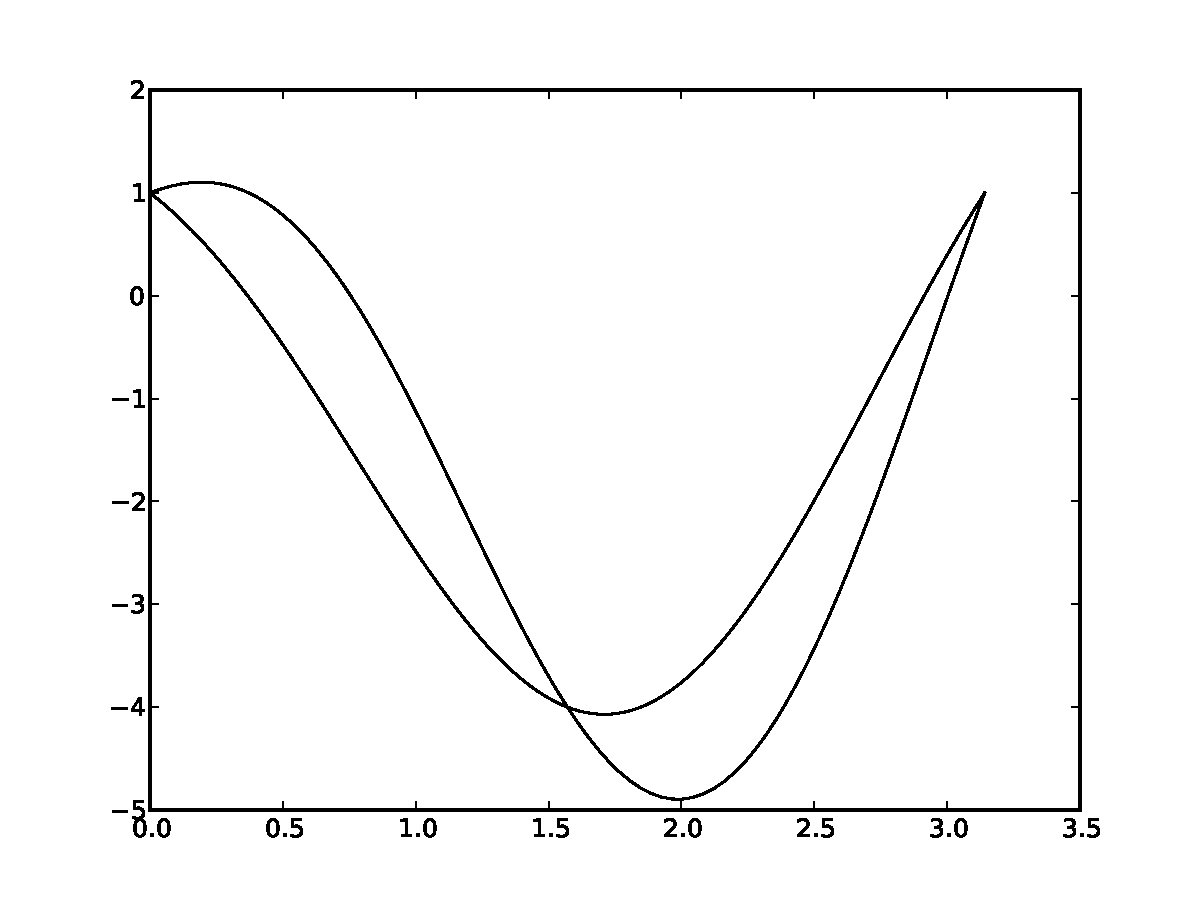
\includegraphics[width=\textwidth]{Fig1.pdf}
\caption{Two solutions of $y'' = -4y -9\sin(x),$ both satisfying the boundary conditions $y(0) = y(\pi) = 1.$}
\label{shooting:prob1}
\end{figure}

Let us consider how to solve for $\frac{d}{dt} y(b,t)$. We will assume that the function $y(x,t)$ can be differentiated with respect to $x$ and $t$ in any order, and let  $z(x,t) = \frac{d}{dt} y(x,t).$ Using the chain rule, we obtain 
\begin{eqnarray*}
z'' = \frac{d}{dt} y''(x,t) &=& \frac{\partial f}{\partial y} (x,y(x,t),y'(x,t)) \cdot \frac{dy}{dt}(x,t) ,\\
&+& \frac{\partial f}{\partial y'} (x,y(x,t),y'(x,t)) \cdot \frac{dy'}{dt}(x,t),
\end{eqnarray*}
Using the initial conditions associated with $y(x,t)$, we obtain the following initial value problem for $z(x,t)$: 
\begin{eqnarray*}
z'' &=& \frac{\partial f}{\partial y} (x,y,y') z + \frac{\partial f}{\partial y'} (x,y,y') z'
,\,\,a \leq x \leq b, \\
 z(a) &=& 0, z'(a) = 1.
\end{eqnarray*}

To use Newton's method, the (coupled) IVPs for $y$ and $z$ must be solved simultaneously. The iterative method then becomes 
\[
t_{n+1} = t_n - \frac{ y(b,t_n) - \beta}{z(b,t_n)}, \,\, n = 0,1,\hdots
.\]


\begin{problem}
Use Newton's method to solve the bvp
\begin{equation*}
\begin{split}
y'' &= 3 + \frac{2y}{x^2}, \,\, x \in [1,e],\\
y(1) &= 6, \\
y(e) &= e^2 + 6/e.
\end{split}
\end{equation*}
Plot your solution. (Compare with Figure \eqref{shooting:prob2}.) What is an appropriate initial guess? 
\end{problem}


\begin{figure}[ht]
\centering
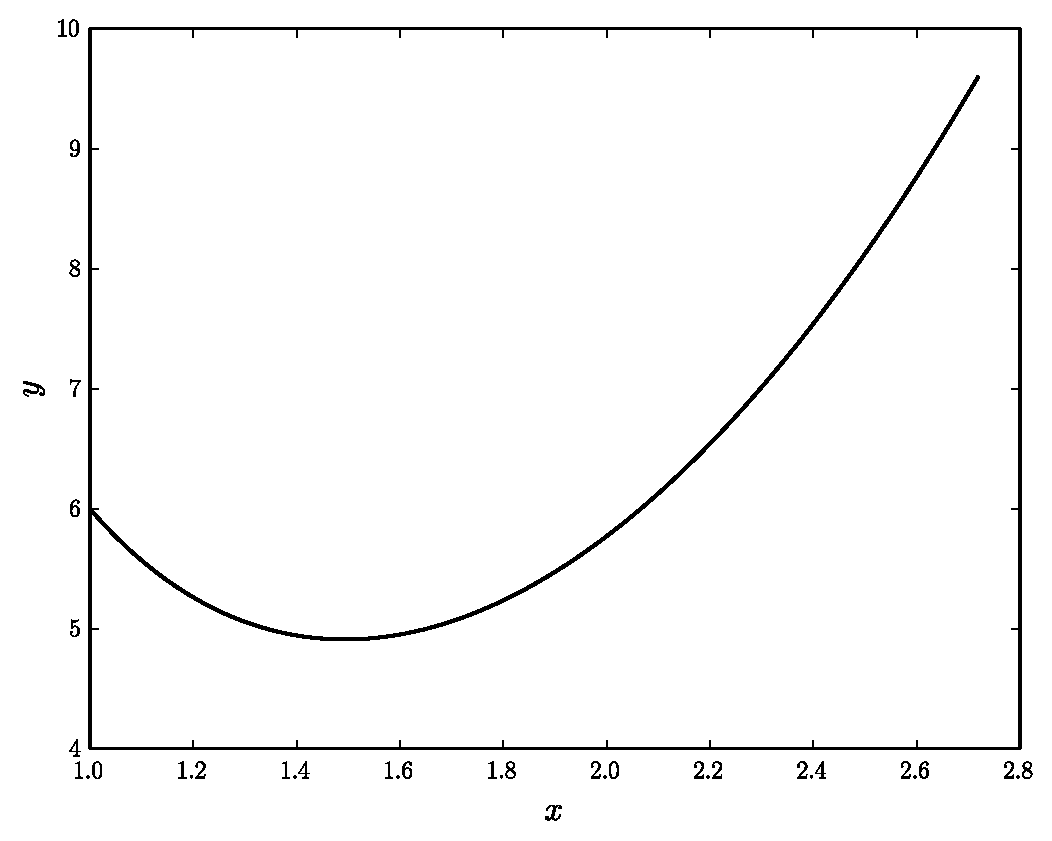
\includegraphics[width=\textwidth]{Fig2.pdf}
\caption{The solution of  $y'' = 3 + 2y/x^2,$ satisfying the boundary conditions $y(1) = 6$, $ y(e) =  e^2 + 6/e$.}
\label{shooting:prob2}
\end{figure}

% \pagebreak

\section{The Cannon Problem}

Consider the problem of aiming a projectile at a given target. Here we will construct a differential equation that describes the path of the projectile and takes into account air resistance. We will then use the shooting method to determine the angle at which the projectile should be launched. 

Let the coordinates of the projectile be given by $\vec{r}(t) = \langle x(t), y(t) \rangle.$ If $\theta(t)$ represents the angle of the velocity vector from the positive $x$-axis and $v(t)$ represents the speed of the projectile ($ |\vec{v}(t) |$), then we have 
\begin{align*}
\dot{x} &= v\cos{\theta},\\
\dot{y} &= v\sin{\theta}.\\
\end{align*}
The tangent vector to the path traced by the projectile is the unit vector in the direction of the projectile's velocity, so $\vec{T}(t) = \langle \cos{\theta}, \sin{\theta} \rangle.$ The unit normal vector $\vec{N} (t)$ is given by $\vec{N} (t)= \langle -\sin{\theta}, \cos{\theta} \rangle.$ Thus the relationship between basis vectors $\vec{i}, \vec{j}$, and $\vec{T(t)}, \vec{N}(t)$ is given by 

\[
\left[\begin{array}{cc}\cos{\theta} & \sin{\theta} \\-\sin{\theta} & \cos{\theta}\end{array}\right] \left[\begin{array}{c}\vec{i} \\\vec{j}\end{array}\right] = \left[\begin{array}{c}\vec{T(t)} \\\vec{N(t)}\end{array}\right]
.\]


Let $F_g$ represent the force on the projectile due to gravity, and $F_d$ represent the force on the projectile due to air resistance. (We assume the air is still.) From Newton's law we have
\begin{align*}
m \dot{\vec{v}} &= F_g + F_d.
\end{align*}

The drag equation from fluid dynamics says that the force on the projectile due to air resistance is $k v^2 = (1/2)\rho c_D A v^2$, where $\rho$ is the mass density of air (about $1.225$ $\text{kg}/\text{m}^3$), $v$ is the speed of the projectile, and $A$ is its cross-sectional area.  The drag coefficient $c_D$ is a dimensionless quantity that changes with respect to the shape of the object. (If we assume our projectile is spherical with a diameter of $.2$ m, then its drag coefficient $c_D \approx 0.47$, its cross-sectional area is $\pi/100$ $ \text{m}^2$, and we obtain $k \approx 0.009.$ )


Thus the total force on the shell is 
\begin{align}
m \dot{\vec{v}} &= -mg \vec{j} - kv^2 \vec{T},\nonumber \\
&= -mg( \sin{\theta} \vec{T} + \cos{\theta} \vec{N} ) - kv^2 \vec{T},\nonumber\\
&= (-mg \sin{\theta} - k v^2 ) \vec{T} - mg \cos{\theta} \vec{N}.\label{TForce1}
\end{align}
From the identity 
$\vec{v} = \langle \dot{x}, \dot{y} \rangle = \langle v \cos{\theta}, v \sin{\theta} \rangle$ 
we have 
\begin{align}
m \dot{\vec{v}} = {} & m\langle v' \cos{\theta} - v\sin{\theta} \cdot \theta' ,v'\sin{\theta} + v\cos{\theta} \cdot \theta' \rangle \nonumber \\
= {} & m(v'\cos{\theta} - v\sin{\theta} \cdot \theta')(\cos{\theta} \vec{T} - \sin{\theta}\vec{N}) \nonumber \\
& + m(v' \sin{\theta} + v\cos{\theta} \cdot \theta')( \sin{\theta} \vec{T} + \cos{\theta} \vec{N}) ,  \nonumber \\
= {} & m(\vec{T} \cdot v' + \vec{N} \cdot v \cdot \theta') . \label{TForce2}
\end{align}
From equations \eqref{TForce1} and \eqref{TForce2} we have 
\begin{align*}
mv' &= -mg\sin{\theta} - k v^2,\\
mv\theta' &= -mg \cos{\theta}.
\end{align*}
Thus we have the coupled system of differential equations
\begin{align}
\dot{x} &= v\cos{\theta}, \nonumber \\
\dot{y} &= v\sin{\theta},\nonumber \\
v' &= -g\sin{\theta} -  k v^2/m,\nonumber \\
\theta' &= -g \cos{\theta}/v. \nonumber
\end{align}


The independent variable $t$ used above is unessential to our problem. If we assume that $t$ is an smooth invertible function of $x$ ($t = t(x)$), then we obtain 
\begin{align*}
\frac{dy}{dx} &= \frac{dy}{dt}\frac{dt}{dx} ,\\
&= \frac{dy}{dt} \frac{1}{v\cos{\theta}}, \\
&= \frac{v \sin{\theta}}{v\cos{\theta}} = \tan{\theta}.
\end{align*}
We find $\frac{dv}{dx}$ and $\frac{d\theta}{dx}$ in a similar manner. 
Thus our system of differential equations becomes 
\begin{align}
	\begin{split}
\frac{dy}{dx} &= \tan {\theta} ,\\
\frac{dv}{dx} &= -\frac{g \sin{\theta} + \nu v^2}{v \cos{\theta}},\\
\frac{d\theta}{dx} &= -\frac{g}{v^2}, \label{cannon_DEs}
	\end{split}
\end{align}
where $\nu = k/m.$ In the next problem we will assume that the projectile has a mass of about $60$ kg, so that $\nu \approx .0003$.



\begin{problem}
Consider the following scenario: suppose a projectile is fired from a cannon with velocity $45\text{ m/s}^2.$ At what angle $\theta(0)$ should it be fired to land at a distance of $195\text{ m}$? 

There should be two initial angles $\theta(0)$ that produce a solution for this bvp. Use the secant method to numerically compute and then plot both trajectories.
\begin{align}
	\label{cannon_shooting}
	\begin{split}
\frac{dy}{dx} &= \tan {\theta} ,\\
\frac{dv}{dx} &= -\frac{g \sin{\theta} + \nu v^2}{v \cos{\theta}},\\
\frac{d\theta}{dx} &= -\frac{g}{v^2},\\
y(0)&= y(195) = 0,\\
v(0) &= 45 \text{ m/s}^2.
	\end{split}
\end{align}
($g = 9.8067\text{ m/s}^2.$) Find both solutions for this boundary value problem when $\nu = .0003$. Compare with the solutions when $\nu = 0.$ Their graphs are given in Figure \eqref{shooting:cannon_comparison}.

Hint: This is a system of three first order differential equations, and so our secant method requires a slight modification. Define an appropriate function $f(t)$. 
\end{problem}

\begin{figure}[ht]
\centering
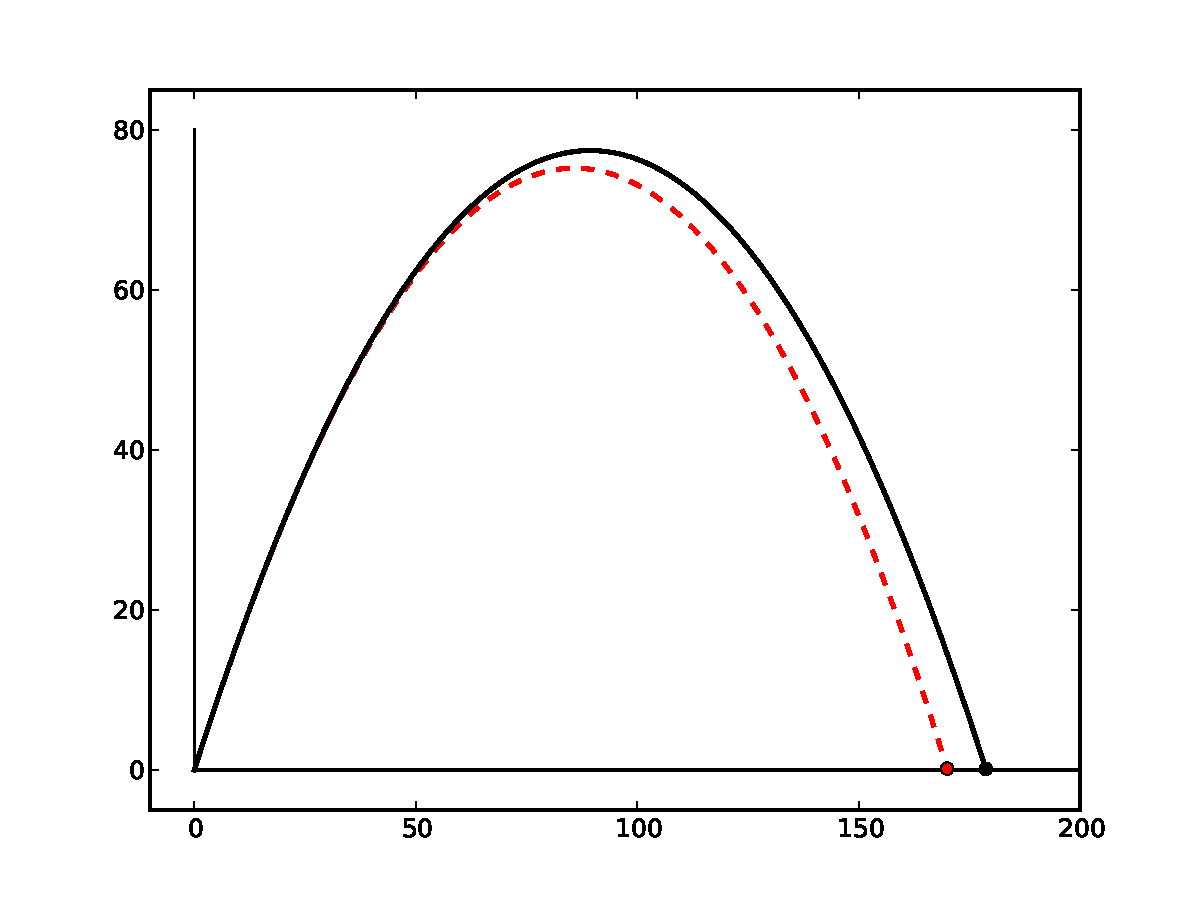
\includegraphics[width=\textwidth]{Cannon_with_AirResistance.pdf}
\caption{Two solutions of the system of equations \eqref{cannon_DEs}, both with initial conditions  $y(0) = 0 \text{ m},$ $ v(0) = 45 \text{ m/s},$ and $\theta(0)=\pi/3$. The black curve is the trajectory of a projectile immune to air resistance ($\nu = 0$). The red curve describes the trajectory of a more realistic projectile ($\nu = .0003$). }
\label{shooting:cannon_comparison}
\end{figure}


\begin{figure}[ht]
\centering
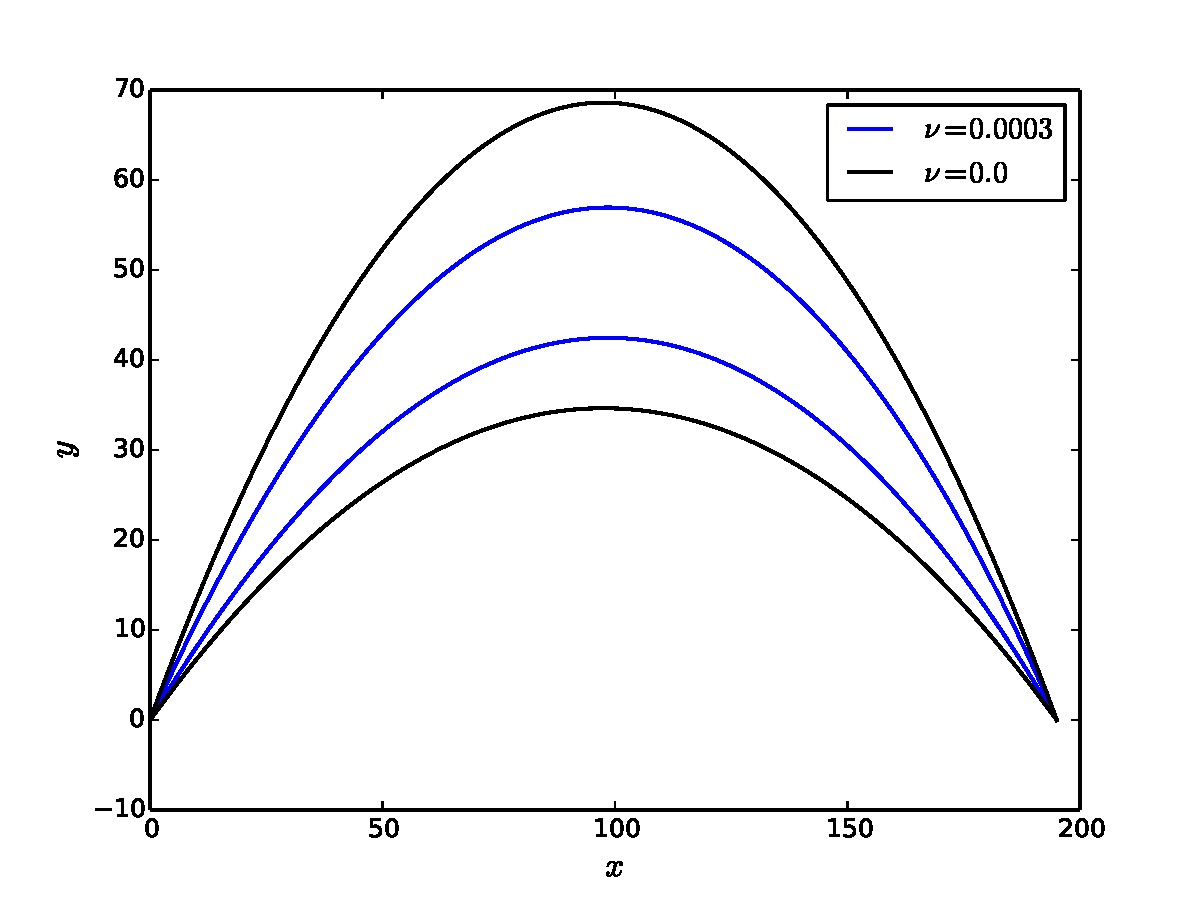
\includegraphics[width=\textwidth]{Cannon_Shooting.pdf}
\caption{Two solutions of the boundary value problem \eqref{cannon_shooting} when the air resistance is described by the parameter $\nu = .0003$. Also both solutions when air resistance is not described in the model ($\nu = 0$).}
\label{shooting:cannon_comparison}
\end{figure}





